%----------------------------------------------------------------------------
\section{Távközlő hálózatok}
{\footnotesize Fizikai jelátviteli közegek. Forráskódolás, csatornakódolás és moduláció. Csatornafelosztás és multiplexelési technikák. Vezetékes és a mobil távközlő hálózatok. Műholdas kommunikáció és helymeghatározás.}
%----------------------------------------------------------------------------
\subsection{Fizikai jelátviteli közegek.}

\subsubsection{alapfogalmak}
\paragraph{Csatorna maximális adatátviteli rátája | sebessége (C)} Ha a (zajtalan) csatorna $V$ darab diszkrét érték (jelszint) elkülönítésére képes, akkor:
$$C=2H\cdot \log_{2}V$$
ahol $C$ a max átviteli ráta bit/s-ban, $H$ a csatorna sávszélessége Hz-ben és V a jelszintek száma szintén Hz-ben.

\paragraph{Vonali zaj} Az átviteli közeg környezetéből származó energia csomagok. Az átvitt jelek csillapítása miatt a zajszint összemérhetővé válhat a jelszinttel, és a jelek helyes érzékelése nehezebb lesz. Az átviteli közegek jellemezhetőek az átlagos jelteljesítmény (Signal) és zajteljesítmény (Noise) hányadosával ($\frac{S}{N}$). Általában dB skálán mérjük.
Max adatátviteli sebesség zajos csatornára:
$$ C=H\cdot\log_{2}(1+ \frac{S}{N})$$

\paragraph{Csillapítás (A--Attenuation)} A jel amplitúdója csökken a haladása során az átviteli közegben. Emiatt a közegek hosszát úgy állapítják meg, hogy a jel biztonsággal értelmezhető legyen a vételi oldalon. Nagyobb távolságra erősítők (jelismétlők) beiktatásával kell a jelet visszaállítani. A csillapítás frekvenciafüggő, ezért az erősítőknek frekvenciafüggő erősítéssel kell ezt kompenzálniuk. Mértékegysége: dB (decibell)
$$ A = 10\cdot\log_{10}\frac{P_R}{P_T}$$
ahol $P_R$ a vételi oldal teljesítménye, $P_T$ a küldési oldal teljesítménye.
\paragraph{Jelterjedési sebesség} A forrásból küldött energia csomag (impulzus) terjedési sebessége a közegtől és a jel tartományától függ. $v=\lambda\cdot f$ azaz a sebesség a frekvencia és a hullámhossz szorzata.

\subsubsection{Koaxiális kábel}
A középponttól a burkolatig haladva az alábbi részekből áll: központi vezeték, dielektrum, árnyékoló réteg, külső műanyag szigetelés.\\
A koncentrikus felépítés miatt kevésbé érzékeny a zavarokra és az áthallásra, mint a csavart érpár. Nagyobb távolságra használható és többpontos alkalmazásban több állomást is képes támogatni (egy közös vonalon).

Egy vezetékre párhuzamosan több kommunikációs eszköz is felszerelhető. 
Analóg átvitel esetén néhány km-enként szükséges erősítés. Mintegy 600 MHz-ig
használható. Digitális átvitel esetén km-enként szükséges jelismétlő használata.
A mai (strukturált kábelezési technológiára épülő) LAN környezetekben már nem
használják új építésű passzív hálózatokhoz.

\subsubsection{Csavart érpár}
A távközlésben alkalmazott kábeltípusok több csavart érpárt tartalmaznak (Számítógép hálózatoknál a 4 érpár szokott lenni). Ezek egy része oda másik része visszirányú információtovábbításra szolgál.

A csavart érpárú kábeleket többféleképpen csoportosíthatjuk. Egyik alapvető különbsége a kábeleknek az árnyékolásuk. Eszerint léteznek árnyékolatlan (UTP), és árnyékolt (FTP,STP) kábeltípusok. Ezen túlmenően a kábelek átviteli jellemzők szerint különböző kategóriákba csoportosítjuk őket:\\
\begin{tabular}{|c|c|c|c|}
	\hline 
	Kategória (USA) & Osztály (EU) & Frekvencia & Bitráta \\ 
	\hline 
	Caetgory 3 & Class C & 16 MHz & 10 Mb/s \\ 
	\hline 
	Cat. 5/5e & Class D & 125 MHz & 100 Mb/s 2 ill. 1 Gb/s 4 érpáron \\ 
	\hline 
	Cat 6 & Class E & 250 MHz & 1 Gb/s 2 érpáron \\ 
	\hline 
	Cat 6a & Class EA & 500 MHz & 10 Gb/s \\ 
	\hline 
	Cat 7 & Class F & 600 MHz & 10 Gb/s \\ 
	\hline 
\end{tabular} 

A csavart érpár kialakításával két dolgot érünk el:
\begin{description}[nosep]
	\item[Zajcsökkentés] A külső zavaró jelek a két, egymáshoz közeli és azonos tulajdonságú dróton megegyező amplitúdóval és fázissal jelennek meg, így a két drót közötti feszültségben a külső jelek hatása nagymértékben kioltja egymást. A csavarásnak köszönhetően a két drót hasonlóan erősen csatolódik a külső jelekhez, hiszen néha az egyik, néha a másik drót van közelebb a zavaró jel forrásához. (Emiatt kell több érpárt más menetemelkedéssel csavarni, hogy ne legyenek minden menetben ugyanúgy összecsatolódva a különböző párok tagjai. Az áthallás így minimalizálható.)
	\item[Vezeték sugárzásának csökkentése] A pár két tagján ellentétes fázisú jelet továbbítva a két drót sugárzása erősen kioltja egymást, így nem fog antennaként viselkedni a kábel.
\end{description}

\subsubsection{Optikai szál}
Az optikai szálban a jel fényimpulzusok formájában terjed. Nagy adatátviteli ráta és alacsony jelcsillapítás jellemzi (Gb/s több 10 km-en) a galvanikus közegekhez képest. Külső sugárzás nem jut be a szálba, ezért zajtól nem kell tartani, továbbá kifelé sem sugároz emiatt nem lehet zajforrás, nem jelentkezik áthallás. Egy optikai kábel több szálból tevődik össze, melyek hierarchikusan rendezett nyalábokba vannak szervezve. Épületekben, géptermekben oda-vissza irányú szálpárból (egyenként egycsatornásak) alkotott optikai vezetékeket is használnak. A szálak rétegből tevődnek össze: mag, védőburkolat, puffer, köpeny.

Egy optikai szál egy vagy több optikai csatorna (WDM) számára használható. Egy csatornás változatban az oda-vissza pont-pont kapcsolathoz két szál szükséges. A fény egy vagy több módusban terjed az optikai szálban eszerint beszélünk egy-módusú (SMF--Singlemode Fibre) és több-módusú (MMF--Multimode Fibre) optikai szálról. Fizikai megnyilvánulásaikban az SMF kábel magja kisebb keresztmetszetű az MMF-éhez képest. Jeltovábbítás tekintetében az SMF jobb, mivel a fény a szál tengelyével párhuzamosan fut visszaverődés nélkül. Emiatt a fényimpulzusok nem torzulnak, nagyobb átviteli sebesség érhető el.

\subsubsection{Rádióhullámok}
A rádióhullámok térben egyetlen periodikus jel vagy több periodikus jel összege. A kiküldött jel ugyanúgy csillapodik a térben, mint más anyagi közegek esetében, ezért hatótávolságon belül alkalmazható. Az elektromágneses tér igen zajos, a környezeti elektromágneses jelenségek más adók erősen befolyásolják a csatorna minőségét. A rádióhullámú technikákat többféle szempont szerint osztályozhatjuk:
\begin{easylist}[enumerate]
	# Lefedett fizikai terület
	## Irányított: két csomópont menti egyenes mentén
	## Szektor: Térszögön belül
	## Minden irányba: teljes térszögben
	# Frekvencia komponensek száma
	## Alapsávú (baseband): szűk frekvenciatartomány (n=1)
	## Keskenysávú (narrowband): kis frekvenciatartomány (n kicsi)
	## Szélessávú (broadband): tág frekvenciatartomány (n nagy)
	# Alkalmazó kommunikációs technológiák:
	## Távközlés (GSM,LTE,5G,\dots)
	## Adathálózatok (WiMax,WiFi,Bluetooth,RFID,NFC,\dots)
\end{easylist}

\subsection{Forráskódolás, csatornakódolás és moduláció.}
\begin{figure}[h]
	\centering
	
\includegraphics[width=0.5\linewidth]{fig/12-hirkozlesi_rendszer}
	\caption{Egy tetszőleges hírközlési rendszer}
	\label{fig:12-hirkozlesirendszer}
\end{figure}
\begin{figure}[h]
	\centering
	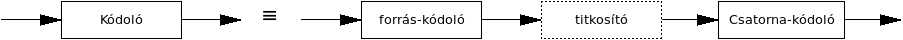
\includegraphics[width=0.7\linewidth]{fig/12-kodolo_felepitese}
	\caption{Kódoló felépítése (dekódoló ehhez hasonló)}
	\label{fig:12-kodolofelepitese}
\end{figure}

\begin{definition}{Kódolás}
	A közlemények(végtelen) halmazából a kódközlemények(végtelen) halmazába képző függvény.
\end{definition}
\begin{note}
	Közlemények a forrásból származó a forrásábécé jeleiből (forrásjelek) képzett tetszőleges véges sorozat. A kódközlemény a csatornán haladó a csatornaábécé jeleiből (kódjelek) képzett tetszőleges véges sorozat.
\end{note}
\paragraph{Forráskódolás} az a kódolási eljárás, amikor az a cél, hogy a kódközlemény minimális redundanciával rendelkezzen. Tehát cél a gazdaságosság és általában ez egyértelmű dekódolhatóság!

\paragraph{Csatornakódolás} Cél a közlemény megbízható átvitele a csatornán, emiatt az egyes kódközlemények redundanciával rendelkeznek. A redundanciát a hibajelző és hibajavító kódolások okozzák.

\paragraph{Moduláció} A (digitális)kódjelek fizikai analóg jelekre történő leképzése. Gyakran hívják a fizikai jelzéseket egyszerűen jeleknek, míg a forrásjeleket és kódjeleket (forrás- és kód) karaktereknek vagy szimbólumoknak.


\paragraph{Jelkódolás} A (digitális) adat leképezése (digitális) vivőjelre (pl. feszültségszintekre, feszültségszint-váltásokra). A fizikai rétegben megjelenős bitsorozatot az alkalmazott csatorna jelkészletére, jelzésrendszerére képezzük le.

\paragraph{Moduláció sebesség (jelváltás sebesség)} Időegység alatt bekövetkező jelváltások száma, vagyis a csatornán érvényes szimbólumok közötti átmenetek száma. Mértékegysége: jelváltás/másodperc (baud)\\
A modulációsebesség és az adatátviteli sebesség (természetesen) különböző mennyiségek mérésére szolgál, de egy konkrét, jól meghatározott környezetben a két mennyiség között szoros összefüggés áll fenn.

\subsubsection{Forráskódolás}
\paragraph{Huffmann--féle optimális kód}
A Huffman-kódolás karakterek (jelek, betűk, számjegyek) olyan kódolását jelenti, amelyben az egyes kódok nem azonos hosszúságúak (különböző számú bitből állnak) annak érdekében, hogy a szövegek átlagosan rövidebbek legyenek, mint az azonos hosszúságú kódok használata esetében. Ez a karakterek gyakoriságának figyelembe vételével történik. A kódolás egy mohó stratégián alapszik, és az adattömörítésben igen hatékonyan használható. Hasonlóan változó kódszóhosszúgású kódolás még a Shannon--féle kódolás, ill. a Gilbert-féle kód, melyeknél a gyengébb optimalizálás árán gyorsabban végrehajtható algoritmust alkalmazunk.

\paragraph{Lempel-Ziv kódolás}
Adattömörítési feladatoknál gyakorta alkalmazott. A tömörítés alapja, hogy a kódoló csak egy szótárbeli indexet küld át. A szótár dinamikusan bővül, kiinduló állapotban az összes egybetűs szimbólumot tartalmazza. A kódolás elve igen egyszerű: az aktuális pozíciótól kezdve addig kell a szimbólumokat kiolvasni, amíg a sorozat szerepel a szótárban. Ezután elküldjük ezen sorozat indexét, a szótárba felvesszük kiegészítve a következő szimbólummal, és az algoritmust ettől a szimbólumtól folytatjuk.


\subsubsection{Jelkódolási technikák}
\begin{multicols}{2}
\paragraph{NRZ (Non-Return- to Zero) jelkódolás} Legegyszerűbb kódolási technika, könnyen implementálható, de nem biztosít szinkronizációt hosszabb 0 vagy 1 sorozatok esetén.\\
0 bit: alacsony jelszint teljes bitidőben.\\ 
1 bit: magas jelszint teljes bitidőben.\\ 
Jelváltás a bitidő elején történik.

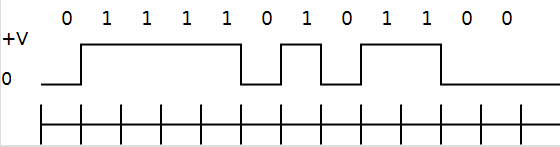
\includegraphics[width=\linewidth]{fig/12-NRZ}
\end{multicols}

\begin{multicols}{2}
\paragraph{RZ (Return to Zero) jelkódolás} Jelváltási sebesség duplikáció csupa 1-es esetén\\
0 bit: alacsony jelszint teljes bitidőben\\
1 bit: első félidőben magas majd alacsony jelszint

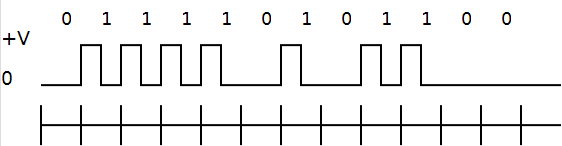
\includegraphics[width=\linewidth]{fig/12-RZ}
\end{multicols}

\begin{multicols}{2}
\paragraph{NRZI (Non-Return to Zero Invert on One) jelkódolás}~\\
0 bit: változatlan jelszint\\
1 bit: jelszint váltás a bitidő elején

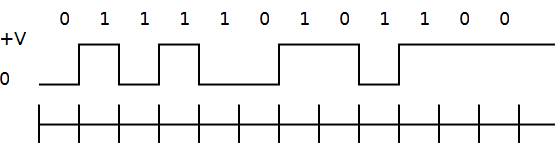
\includegraphics[width=\linewidth]{fig/12-NRZ1}
\end{multicols}

\begin{multicols}{2}
\paragraph{Manchester jelkódolás} A klasszikus Ethernet is használta ezt a kódolást. Folyamatos szinkronizációt biztosít, de dupla jelváltás-sebességet igényel.\\
0 bit: negatív jelátmenet a bitidő felénél\\
1 bit: pozitív jelátmenet a bitidő felénél

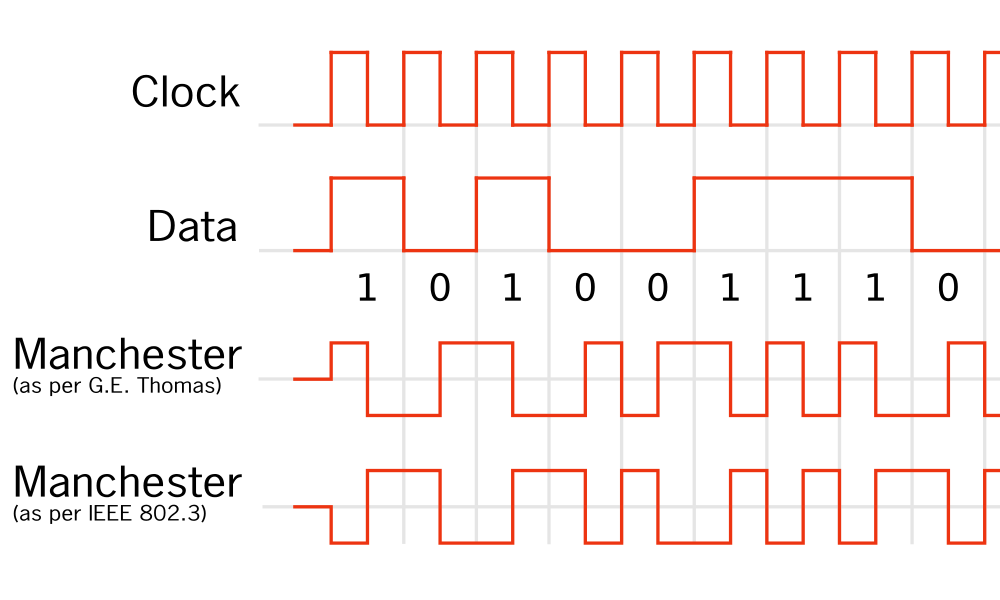
\includegraphics[width=\linewidth]{fig/12_Manchester}
\end{multicols}

\subsubsection{Csatornakódolás}

\paragraph{4B/5B}

\subsubsection{Moduláció}
A bináris információt sok esetben nem alapsávi impulzusok formájában visszük át a csatornán, hanem egy (alsó- és felső frekvenciahatár megadásával) jól meghatározott frekvenciatartománnyal rendelkező (sáváteresztő) csatornán. A rendelkezésre álló frekvenciasáv középértéke adja a vivőfrekvenciát, melyen valamilyen modulációs eljárással tudjuk leképezni a továbbítandó bit értékét.

\begin{multicols}{2}
\paragraph{ASK (Amplitude Shift Keying -- Amplitúdó váltás)} Előnye az egyszerű implementáció. Hátrány a diszkrét komponens jelenléte.\\
0 bit: vivőfrekvencia hiánya (Amplitúdó A=0). $S_{(0)}(t) = 0$\\
1 bit: A amplitúdójú vivőfrekvencia jelenléte. $S_{(1)}(t) = A\cdot\sin(\omega_v\cdot t) $\\
\begin{center}
	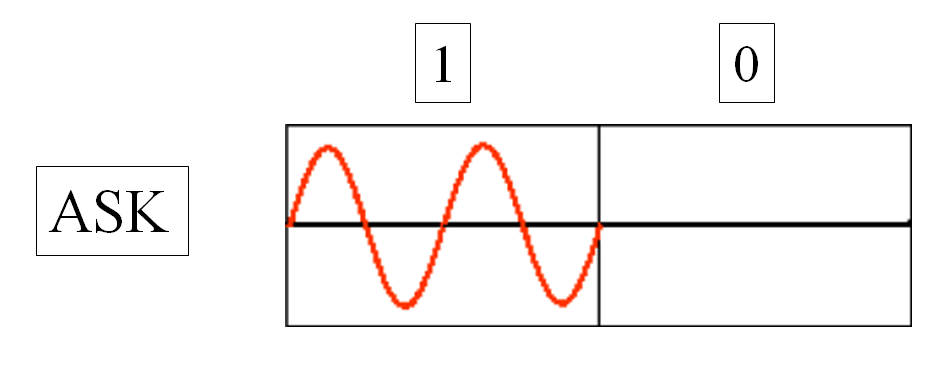
\includegraphics[width=\linewidth]{fig/12-ASK}
\end{center}
\end{multicols}

\begin{multicols}{2}
\paragraph{FSK (Frequency Shift Keying -- Frekvencia váltás)} Előny az egyszerű dekódolás. Hátrány a nagy sávszélesség igény.\\
0 bit: vivőfrekvenciánál $\omega_d$ frekvencialökettel nagyobb frekvencia. $S_{(0)}(t) = A\cdot\sin((\omega_v + \omega_d)\cdot t) $\\
1 bit: vivőfrekvenciánál $\omega_d$ frekvencialökettel kisebb frekvencia. $S_{(1)}(t) = A\cdot\sin((\omega_v - \omega_d)\cdot t) $\\
Itt a bit ráta és a baud ráta értéke azonos. A sávszélesség szükséglet: $2\omega_d$
\begin{center}
	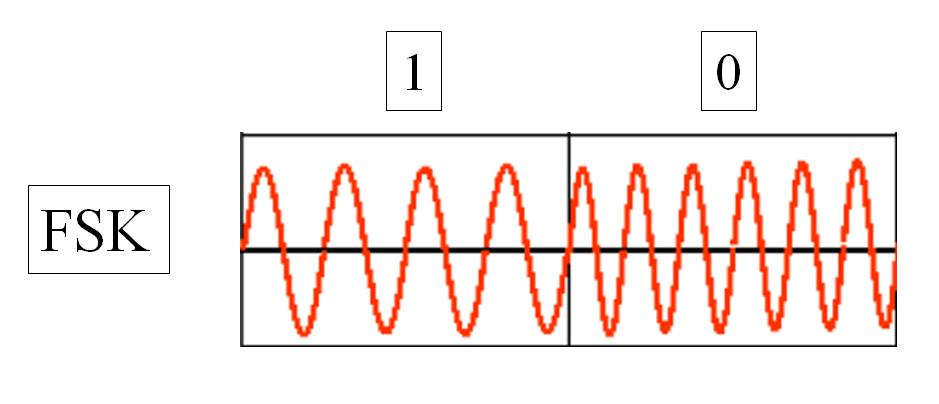
\includegraphics[width=\linewidth]{fig/12-FSK}
\end{center}
\end{multicols}

\begin{multicols}{2}
\paragraph{PSK (Phase Shift Keying -- fázis váltás)} ~\\
0 bit: a vivőhöz képest ellentétes fázisú jel. $S_{(0)}(t) = A\cdot\sin((\omega_v)\cdot t+\pi)= -A\cdot\sin((\omega_v)\cdot t) $\\
1 bit: a vivővel azonos fázisú jel. $S_{(1)}(t) = A\cdot\sin((\omega_v)\cdot t)$\\
Ez a felírási forma általánosítási lehetőséget nyit a többszintű PSK alkalmazására: 180 fok helyett több kisebb eltolási érték segítségével egy átviteli időegységben több bit átvitele is megoldható.
Pl.: 4 szintű PSK (Quadrate PSK, QPSK): 0, 90, 180 és 270 fokos eltolások léteznek. Itt egy időegység alatt két bitnyi információ vihető át.
\begin{center}
	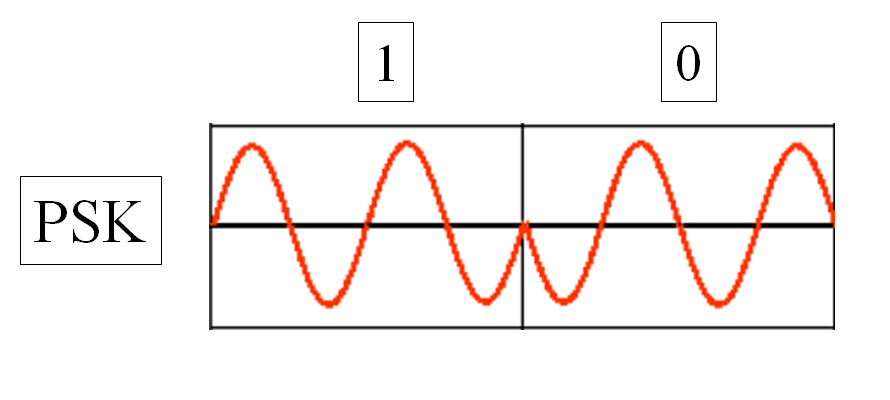
\includegraphics[width=\linewidth]{fig/12-PSK}
\end{center}
\end{multicols}

\paragraph{QAM (Kvadratúra amplitúdómoduláció)}
Egy jelet meghatároz a vivőjelhez képest mért amplitúdó és fáziseltolás mértéke. Ezáltal egyetlen jel több bitnyi információt közvetít. Attól függően, hogy hány különböző érvényes jelet tartalmaz beszélhetünk 4-QAM (2 bites), 8-QAM (3 bites), 16-QAM (4 bites), stb\dots modulációkról, melyek közül a 256-QAM képes egy teljes bájtot kódolni. Minél több különálló jelünk van, annál érzékenyebb az átvitel a zajra, illetve a csillapítás mértékére.
\begin{center}
	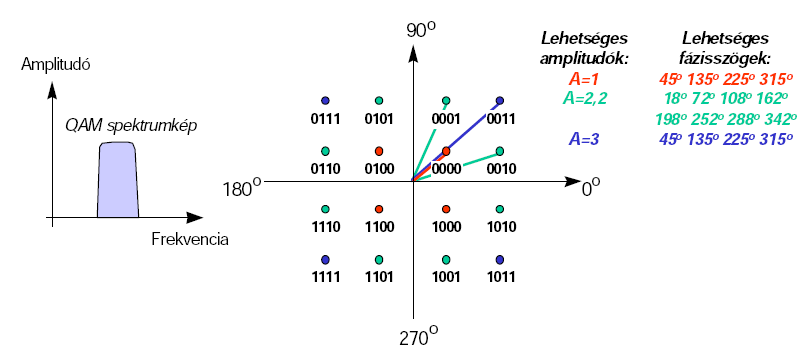
\includegraphics[width=0.7\linewidth]{fig/12-QAM}
\end{center}


\subsection{Csatornafelosztás és multiplexelési technikák.}
Amikor Több forrás kíván ugyanazon a csatornán osztozni szét kell tudnuk választani az egyes forrásokból érkező közleményeket, elkerülendő az üzenetek ütközése illetve az egyes üzenetek azonosítása. Multiplexálás során az egy közös csatornát logikai csatornákra bontjuk, illetve de-multiplexálással szétválogatjuk az üzeneteket.

Multiplexálás alatt a telekommunikációban azt az eljárást értik, amikor két vagy
több csatornát összefognak egy csatornába úgy, hogy az inverz multiplexelés művelettel, vagy demultiplexeléssel, vagy demuxálással elő tudják állítani az eredeti csatornákat. Az eredeti csatornák egy úgynevezett kódolási sémával azonosíthatóak. A multiplexelés kifejezésnek általában a magyar keverés kifejezést feleltethetjük meg. 

Az elektronikus kommunikációban , két alap multiplexelés használatos: az időosztásos multiplexelés (Time-Division Multiplexing -- TDM) és a frekvenciaosztásos multiplexelés (Frequency-Division Multiplexing -- FDM). Az
optikai közeget használó kommunikációban az FDM a hullámhossz-osztásos multiplexelést (Wavelength-Division Multiplexing -- WDM) jelenti.


\subsection{Vezetékes és a mobil távközlő hálózatok.}
\subsubsection{Analóg telefonhálózatok}
Hanghullámok átvitele elektromos hálózaton. Az érthető beszédhez elegendő 0,3-3,4~kHz, ezért egy beszédcsatorna 4~kHz (3,1~kHz + védősáv). A csatornákat frekvenciaosztásos multiplexálással (FDM) oldották meg régen. 10000 beszédcsatornához 40~MHz sávszélesség szükséges, de a hierchikus szervezés miatt további védősávok kellenek így 60~MHz a sávszélesség, ami egyetlen koaxiális kábelen átvihető. Az FDM-mel valós áramkörkapcsolás valósul meg.

\subsubsection{Digitális telefonhálózatok}
Mivel a végberendezések jobbára analóg eszközök, ezért A/D D/A átalakítókra van szükség, amit a helyi kapcsolóközpontokban valósítanak meg. Ilyen rendszereknél időosztásos multiplexálással (TDM) működnek. Ez még mindig valós áramkörkapcsolást jelent. Az analóg jelek digitalizálás PCM (Pulse Coded Modulation) kódolással történik.


\paragraph{PCM} A mintavételezés sűrűsége kétszerese a frekvenciának. Egy minta a hullám aktuális amplitúdója a mintavételezés időpontjában. Beszélhetünk lineáris és nemlineáris kvantálásról attól függően, hogy az egyes amplitúdó értékek kvantálási intervallumai megegyeznek-e.

Digitális telefónia esetén egy csatorna sávszélessége 64~kHz.

\paragraph{ADSL -- Asymmetric Digital Subscriber Line} Telefónia és adatátvitel egyidejűleg. Az ADSL lényege, hogy a meglévő távbeszélő (vagy ISDN) alapszolgáltatással párhuzamosan, ugyanazt az előfizetői érpárat felhasználva kapcsolatot biztosítson a nagysebességű hálózatokhoz.
Az ADSL jellemzője a DSL megoldásokon belül, hogy a letöltési és a feltöltési sávszélesség aránya nem egyenlő (vagyis a vonal aszimmetrikus), amely az otthoni felhasználóknak kedvezve a letöltés sebességét helyezi előnybe a feltöltéssel szemben, általában 8:1 arányban. Mind technikai, mind üzleti okai vannak az ADSL gyors elterjedésének. A technikai előnyt az adja, hogy a zajelnyomási lehetőségeket kihasználva lehetővé teszi nagyobb távolságon is a gyors adatátvitelt. Az első generációs ADSL letöltési sebessége 256~kbit/s-tól indul és 8096~kbit/s-ig emelhető, a feltöltésé 64~kbit/s-től 832~kbit/s-ig állítható. Az ADSL2 névre keresztelt továbbfejlesztés első verziója 12~Mbit/s, majd a néhány hónappal később érkezett ADSL2+ 24~Mbit/s elméleti maximális letöltést tesz lehetővé.

Ahhoz hogy egy-időben, egymástól függetlenül telefon (vagy ISDN) szolgáltatást és kétirányú nagysebességű adatátvitelt biztosítson egy szűrőt (splitter) kell az ügyfélnél és a központ oldalon is elhelyezni. A splitter FDM multiplexálást valósít meg
\subparagraph{Splitter} az előfizetői érpárra kapcsolódik, feladata az alacsonyabb frekvenciájú telefon (vagy ISDN) jelek, és a magasabb frekvenciasávban működő ADSL jelek szétválasztása.

Az előfizetői oldal ADSL modemjét \textbf{ADSL NT}-nek hívjuk (ADSL Network Termination = ADSL hálózatvégződés), míg a hálózati csomópontban találhatók az un. \textbf{DSLAM} egységek (Digital Subscriber Line Access Multiplexer = Digitális előfizetői hozzáférés koncentrátor). A telefónia, feltöltési és letöltési adatvonalakat FDM-mel választják külön:
\begin{itemize}[nosep]
	\item hang: 0-4 kHz
	\item védősáv: 4-25 kHz
	\item feltöltési sáv: 25-160 kHz
	\item letöltési sáv: 200 kHz - 1.1 MHz
\end{itemize}
A felsorolt sávhatárok elvi szinten igaz, mert a gyakorlatban függ a telefonelőfizetéstől (analóg: 4~kHZ, ISDN: 64~kHZ), illetve a fel és letöltési sáv átlapolódhat, továbbá a zaj mértékétől függően egyes frekvenciatartományok nem használhatóak.

\subparagraph{ADSL moduláció} A technológia DMT (Discrete Multitone Modulation) modulációt alkalmazza. Az átvitelre használt frekvenciasávot több, egymás utáni kis sávszélességű csatornára osztjuk (4 kHz), és azokban külön-külön viszünk át hasznos információt. 1,1~MHz $\rightarrow$ 256~csatorna:
\begin{itemize}[nosep]
	\item 0. csatorna -- POTS (hang)
	\item 1-5. csatorna - védősáv (üres)
	\item a megmaradt 250 csatornából 1-1 az upstream és a downstream jelzése
	\item a többi a felhasználói forgalomé. Ha egy csatornán rossz az átvitel, akkor nem használják
\end{itemize}
Az átviteli sebesség függ a vonal átviteli karakterisztikájától és a vonalon lévő zajoktól és zavaroktól (külső zavarok és áthallásból származó zajok)
Minden csatornánál lemérik a jel/zaj viszonyt, ehhez igazodva különböző QAM modulációval viszik át a biteket az egyes csatornákon.
\begin{center}
	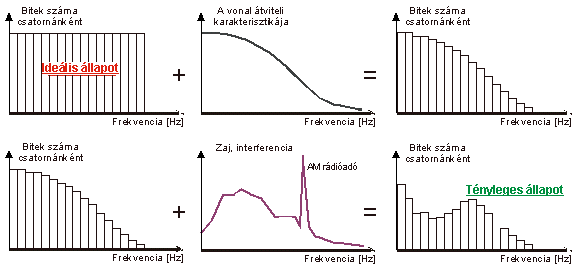
\includegraphics[width=0.7\linewidth]{fig/12-DMT}
\end{center}
\subsubsection{Mobilhálózatok}
Cellaalapú rádiós hálózat. Ezen rendszerek lényege, hogy a lefedendő területet úgynevezett „cellákra” osztják, minden egyes cellában egy bázisállomással. A bázisállomásokat általában valamilyen nagy sávszélességű vezetékes hálózat kapcsolja össze egymással. A cellák méretét az igénybevételtől függően eltérően határozzák meg, városon belül a pár száz méteres átmérőjű cellák dominálnak, míg városon kívül akár 5--10~km-nél is nagyobb távolságú bázisállomásoktól is foghatunk jeleket.

\paragraph{1. generáció}
Az 1.~generációs (1G) hálózatokat az 1980-as években kezdték el üzemeltetni. Ezek mind analóg rendszerek voltak, támogatták a felhasználó számára észrevétlen, automatikus cellaváltást, valamint már eleve úgy tervezték őket, hogy kapcsolhatók legyenek a vezetékes telefonhálózathoz. Európában az NMT (Nordic Mobile Telephony) volt a domináns. Egy nagy hátránya volt, hogy a szabvány kezdeti változata nem írt elő semmiféle titkosítást a beszédátvitelre, így azt, a megfelelő készülék birtokában, bárki lehallgathatta. Ezek a rendszerek alapvetően beszédátvitelre szolgáltak. Gyenge beszédátviteli minőség, kevés szolgáltatásfajta. Viszonylag nagy, 30--50~km átmérőjű cellák.

\paragraph{2. generáció -- GSM/GPRS/EDGE}
Az igazi áttörést a 2.~generációs (2G) hálózatok megjelenése hozta meg. A legfontosabb eltérés az 1G-hez képest a digitális jelátvitel bevezetése. A digitálisan kódolt hangot tömöríteni lehet, így egyszerre sokkal több csatornát lehet használni, mint az ugyanakkora sávszélességet használó analóg rendszerben. A kapacitás további növekedését eredményezte, hogy a digitális mobilkészülékek kisebb teljesítményű rádiót használtak, így a cellák méretét is kisebbre tudták venni. A kisebb teljesítményű rádió kevesebb energiával is beérte, így az akkumulátorok mérete is csökkent. Mindezek sokkal olcsóbbá és hatékonyabbá is tették a mobiltelefonálást. A legelterjedtebb 2G hálózat a GSM. A GSM vezette be az úgynevezett SIM kártyákat. A SIM egy kisméretű írható/olvasható adatkártya, amely tartalmazza a felhasználó hálózaton történő azonosításához szükséges információkat, valamint a telefonkönyvét. Továbbfejlesztés GPRS, EDGE. Rádiós közeghozzáférés: FDMA+TDMA. 900MHz/1800MHz.

\paragraph{3. generáció -- UMTS}
A 3G hálózatok legjelentősebb újításai a 2Ghez képest a megnövekedett kapacitás (több felhasználó kiszolgálása a cellákon belül), a nagysebességű adatkapcsolatok támogatása (internetelérés) és több új hálózati szolgáltatás bevezetése, mint például a videotelefonálás, multimédia szolgáltatások. CDMA közeghozzáférés. HSUPA/HSDPA

\paragraph{4. generáció}
A 4G technológia arra épül, amelyet a 3G kínál, de mindent sokkal gyorsabban hajt végre. MIMO/beamforming. VoLTE.

\paragraph{5. generáció}
IoT eszközök. Nagy sebesség, alacsony késleltetés(ping). Eszköz-eszköz kommunikáció. Okos eszközök, önvezetés.

\subsection{Műholdas kommunikáció és helymeghatározás.}
A műholdas kommunikációs hálózatban a műhold, illetve a hozzá tartozó földi
állomások hálózatot alkotnak. A központi állomások, melyekhez számítógépes
hálózatok, telefon, távíró és egyéb kommunikációs vonalak kapcsolhatók,
eljuttatják az átalakított jeleket a műholdra, amely megváltoztatva a frekvenciát, felerősíti a jeleket és visszajuttatja a földi állomásokra, a felhasználói állomásokra. A távközlési műhold, mint a hálózat legnagyobb egysége a jelek vételére, valamint azok meghatározott területek felé való sugárzására egyaránt alkalmas. Ilyen műholdak keringenek a Föld körül az Intelsat, Eutelsat, Inmarsat stb. rendszerben. 

Egy adott szolgáltatás működtetője a műhold kapacitásából transzponder(rész)t -- csatornát, vonalakat -- bérelhet. A felhasználó a felhasználói állomáson, terminálon keresztül veszi igénybe a rendszer szolgáltatásait. A felhasználói állomások (terminálok) funkciójukat tekintve lehetnek, a) csak vételre szolgáló, illetve b) adó-vevő földi terminálok. A csak vételre szolgáló terminálokkal felépített rendszerek műsor- vagy adatszórásra, tehát egyirányú összeköttetésre alkalmas rendszerek. Egy központi állomásból és csillag alakzatban elhelyezkedő vevőterminálokból állnak. A központ és a terminálok között műholdon keresztül létesül az egyirányú
kapcsolat. A központi állomásból kisugárzott jeleket a műhold közvetítésével
minden, a rendszerbe tartozó (zárt hálózat), vagy az ellátási körzeten belüli
(nyílt hálózat) terminál egyidőben veszi. Erre példa: a francia POLYCOM
rendszer. Az adó-vevő terminálokkal kétirányú, interaktív összeköttetés hozható létre, elsősorban adatátvitel céljából. Tehát a műholdon keresztüli kapcsolat típusa kétféle lehet:
a) egy pont-több pont összeköttetés, amikor a kapcsolat a műholdon keresztül a
központi állomás és az egyes felhasználói állomások (terminálok) között létesül.
b) pont-pont összeköttetés, amikor a kapcsolat két felhasználói állomás (terminál) között létesül.

Felhasználói állomás a tévé- és rádióprogramok vételére alkalmas parabola
antennás műholdvevő is. A 80-as évek nagy szenzációját azonban a VSAT-
terminálok bevezetése jelentette. A VSAT (Very Small Aperture Terminal) nagyon kis méretű antennájú terminált jelent.
A VSAT-rendszer műholdon keresztül létesít a földi terminálok között egy vagy
több irányú, illetve állandó vagy ideiglenes kapcsolatot. A VSAT-rendszer az
OSI referenciamodell 1-3 rétegének kiszolgálásával biztosítja a nyílt rendszerek
szabvány szerinti összekapcsolását.

\subsubsection{GPS}
A GPS (Global Positioning System) Globális Helymeghatározó Rendszer, az
Amerikai Egyesült Államok Védelmi Minisztériuma (Department of Defense)
által (elsődlegesen katonai célokra) kifejlesztett és üzemeltetett -- a Föld bármely pontján, a nap 24~órájában működő -- műholdas helymeghatározó rendszer.
A helymeghatározás 24~db műhold segítségével történik, melyek a Föld felszíne
fölött 20.200~km-es magasságban keringenek, az Egyenlítővel 55~fokos szöget
bezáró pályán. Egy-egy műhold nagyjából naponta kétszer kerüli meg a Földet.
Az égbolton sík terepen egyszerre 7--12 műhold látható, melyből a
helymeghatározáshoz 3, a tengerszint feletti magasság meghatározásához pedig
további egy hold szükséges. A GPS műholdak két frekvencián sugároznak,
ezeket L1-nek (1575,42~MHz) és L2-nek (1227,6~MHz) nevezik. Minden
műhold szórt spektrumú jelet sugároz, amit „pszeudo-véletlen zaj”-nak lehet
nevezni (angol megnevezése: pseudo-random noise, röviden: 'PRN'). Ez a PRN
minden műholdnál különböző. A PRN kódoknak két fajtája van: az első a C/A
(„coarse/acquisition”, a.m. „durva/elérés”), ami ezredmásodpercenként 1023
jelet tartalmaz, a másik kód a P-kód („precision”, a.m. „pontosság”), ami 10230-
at. A C/A kódot az L1 frekvencián adják, a P-kódot mindkét frekvencián. A P-
kódot kizárólag titkos katonai GPS-vevővel lehet dekódolni, ez szabadon nem
hozzáférhető. Értelemszerűen a pontossága nagyobb, mint az általános, polgári
használatra szánt C/A kódnak.

A GPS-rendszert elsősorban rádiónavigációs célokra szánták, azonban emellett
felhasználható a pontos idő és frekvencia terjesztésére is. Minden műholdon két
db. rubídium- vagy cézium-atomóra van elhelyezve. Az oszcillátorok biztosítják
az alapfrekvencia és a kód előállítását is. Az alapfrekvenciát az USDOD földi
állomásai felügyelik, amit egyeztetnek az egyezményes koordinált világidővel
(UTC) (amit az United States Naval Observatory (USNO) állít elő), azonban a
két időfogalom és érték nem azonos egymással. Kölcsönös egyeztetéssel az
USNO és a NIST által előállított UTC-idő 100 ns-on belül (nanoszekundum)
megegyezik egymással, frekvenciaeltérésük kisebb, mint 10-13.

A GPS-idő nem tartalmazza a polgári életben megszokott szökőmásodperceket,
haladása folyamatos, ezért a GPS-vevők megkapják a kettő közötti eltérés
értékét és a készülék a polgári életben használt időt mutatja.

A helymeghatározás elmélete analitikus geometriai módszereken nyugszik. A
műholdas helymeghatározó rendszer időmérésre visszavezetett távolságmérésen
alapul. Mivel ismerjük a rádióhullámok terjedési sebességét, és ismerjük a
rádióhullám kibocsátásának és beérkezésének idejét, ezek alapján meghatározhatjuk a forrás távolságát. A háromdimenziós térben három ismert
helyzetű ponttól mért távolság pontos ismeretében már meg tudjuk határozni a
pozíciót. A további műholdakra mért távolságokkal pontosítani tudjuk ezt az
értéket.